A \emph{iterator} visits entities of a container in a specific 
order and serves as a gernal pointer of the visited entities. 
Iterators in \cgalpoly\ (and \cgalhds) iterate on the 
the primitives of the polyhedron mesh such as halfedges, 
vertices and facets. The visiting order of the iteration
is mostly defined by the storage order of the underlying
container, i.e. the vector or the list. The order
is not dictated by any incidence relationship.
The following example shows how to  on the mesh
vertices.
\begin{lstlisting}
typedef Polyhedron::Vertex_iterator                   Vertex_iterator;

Vertex_iterator vitr, vitr_end = polyhedron.vertices_end();
for(vitr = polyhedron.vertices_begin(); vitr != vitr_end; ++vitr) {
  vitr->doSomething();
}
\end{lstlisting}
Notice the \emph{prefix} increment and decrement is always favored
to postfix. TODO: Refer to \cite{???} for why.
If necessary, \lstinline!Vertex_iterator! is transfomable to the vertex
handle by the assignment. 
\begin{lstlisting}
  Vertex_handle v = vitr;
\end{lstlisting}
Facets and halfedges also have defined iterators in \poly .
\begin{lstlisting}
typedef Polyhedron::Facet_iterator                   Facet_iterator;
typedef Polyhedron::Halfedge_iterator                Halfedge_iterator;

Facet_iterator fitr, fitr_end = polyhedron.facets_end();
for(fitr = polyhedron.facets_begin(); fitr != fitr_end; ++fitr) {
  fitr->doSomething();
}
Halfedge_iterator heitr, heitr_end = polyhedron.halfedges_end();
for(heitr = polyhedron.halfedges_begin(); heitr != heitr_end; ++heitr) {
  heitr->doSomething();
}
\end{lstlisting}

TODO: edge, point and plane iterators. iterator adaptor..

A \emph{circulator} iterates the enities cicularly. 
When a circulator reaches the end, it
starts the iteration again from the begining entity.
Circulators in \cgalpoly\ (and \cgalhds) visits the 
adjacent halfedges of a facet in CCW order and
a vertex in CW order. Different from iterators maintained by 
the polyhedron, circulators are locally associated to
the centered primitive, i.e. facet and vertex. 
Circulators serve as a general pointer of the visited halfedge
and can be transformed to halfedge handles by assignment.
Following codes demonstrate the circulation on the adjacent facets
across the edges surrounding the center facet.

\begin{lstlisting}
typedef Polyhedron::Halfedge_around_facet_circulator Halfedge_facet_circulator;

Halfedge_facet_circulator fcir = f->facet_begin(); // f is a facet handle.
do {
  doSomething(fcir->opposite()->facet());
} while(++fcir != f->facet_begin());
\end{lstlisting}

Circulation on a vertex is similar to a facet except in CCW order.
Following codes demonstrate the circulation of the adjacent vertices
on a vertex in CW order. Note that the decrement of the circulator
forces the traversal in CW order. 
\begin{lstlisting}
typedef Polyhedron::Halfedge_vertex_circulator Halfedge_vertex_circulator;

Halfedge_vertex_circulator vcir = v->vertex_begin(); // v is a vertex handle.
do {
  doSomething(vcir->opposite()->vertex());
} while(--vcir != v->vertex_begin());
\end{lstlisting}

\begin{figure}[htb]
    \centering
    \psfrag{cir}[]{\textbf{cir}}
    \psfrag{++}[]{\textbf{\scriptsize $++$cir}}
    \psfrag{--}[]{\textbf{\scriptsize $--$cir}}
    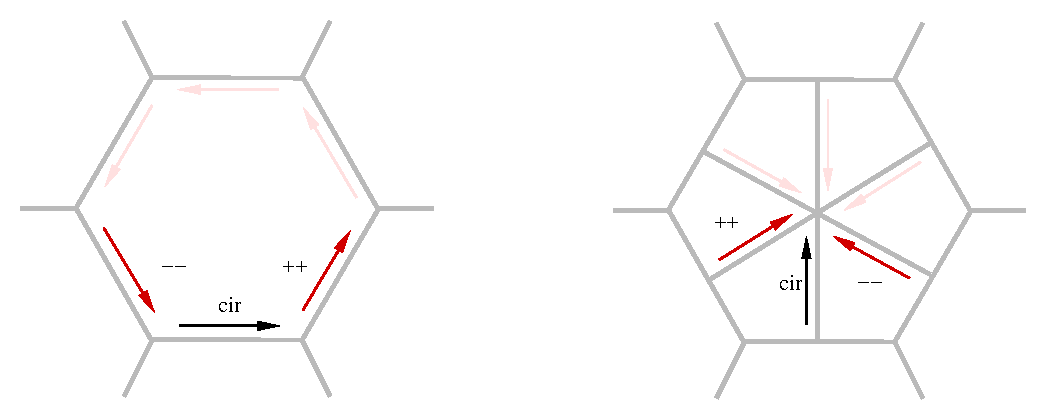
\epsfig{file=pfigs/Circulators.eps, width=12cm}
    \caption{(\IL) circulation around a facet (ccw).
             (\IR) circulation around a vertex (cw).}  
    \label{fig:stl_concept}
\end{figure}


A circulator is mostly used to access the local negorhood (i.e. the 
1-ring region). A unorganized traversal is usually done by the
functions of the adjacency pointers of halfedges, i.e. prev(), next() 
and opposite(). TODO: example.

TODO: useful functions for itr and cir: circulatorsize(), distance(), 
advance(), tranform() ...

